\section{Results}
\label{sec:results}


\subsection{Pixel scale}
Of the \nConfigs{} camera configurations listed in Table~\ref{tab:configs} in the appendix, \nConfigsOwn{} have enough discharges and enough spread in $R_{\rm LCFS}$ for their own fit and cover \nShotsOwnScale{} of the \nShotsProcessed{} processed discharges, while the rest use the pooled slope of their campaign (Figure~\ref{fig:calibration}). The limb-peak column falls linearly with $R_{\rm LCFS}$ in every fitted configuration, with Spearman correlations between \scaleOwnRhoWeak{} and \scaleOwnRhoStrong{}, the sign of every slope agrees with the SOL direction found from the images, and the fitted scales span \scaleOwnMin{}--\scaleOwnMax{}~mm per pixel. The tightest fit is the M6 configuration ``\scaleCfgCampSixView'' (\scaleCfgCampSixN{} discharges, $\rho = \scaleCfgCampSixRho$), at \scaleCfgCampSix{}~mm per pixel (\scaleCfgCampSixLo--\scaleCfgCampSixHi), and the M9 configuration gives \scaleCfgCampNine{}~mm per pixel (\scaleCfgCampNineLo--\scaleCfgCampNineHi). For the same camera, port, and campaign, \citet{farley2019identification} quote a resolution of 5~mm at the tangency plane for wide-angle images reduced to $256 \times 160$ pixels from the $640 \times 448$ mode of the camera, which is about 2~mm per native pixel, so the M9 value is of that order, although 2~mm lies below its interval and the archive does not record whether the lens was the same.

Two features of the calibration limit what the physical units can support, the first being that the intervals are 10--30\% wide and cannot capture a bias common to a whole configuration, such as a drift of the emission peak relative to the LCFS with density. The second is that the filaments look alike in pixel units in every configuration, since across the \nCfgPx{} fitted configurations with at least ten discharges the median track velocity is \vxPxCfgMin{}--\vxPxCfgMax{} pixels per frame and the median width is \fwhmPxCfgMin{}--\fwhmPxCfgMax{} pixels, while the fitted scales differ by a factor of \scaleOwnRatio. The differences between campaigns in Table~\ref{tab:campaigns} therefore reflect differences between their calibrations and are left uninterpreted. Because a scale error multiplies $v_r$ and $\delta_r$ of a configuration by the same factor, it cancels in the velocity--size slopes of Section~\ref{sec:analysis}, which are fitted after each discharge is normalized by its own medians, and it moves a discharge along a diagonal in the regime diagram without changing the conclusions drawn there.

\begin{figure}[t]
\centering
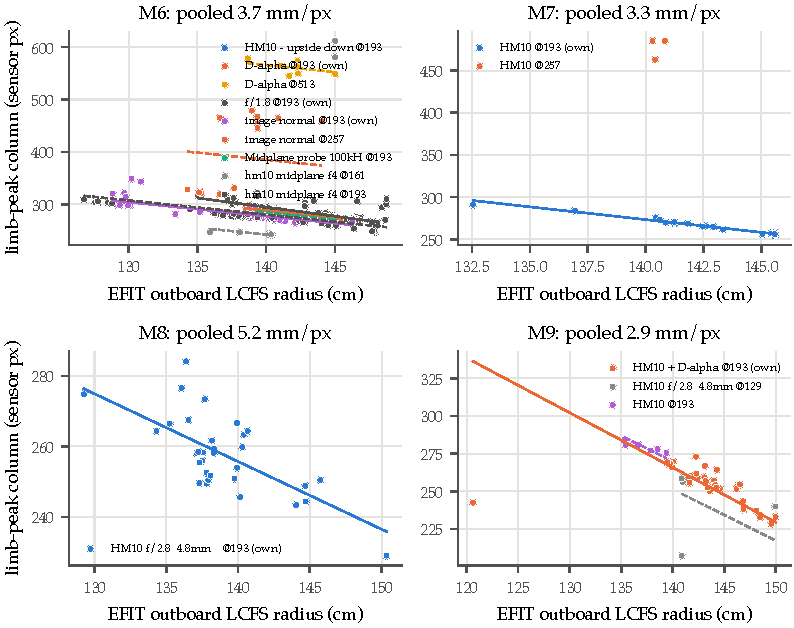
\includegraphics[width=\linewidth]{figs/fig_calibration.pdf}
\caption{Between-shot pixel-scale calibration, in which each point is one discharge, placed at its median limb-peak column in sensor coordinates over the flat top against its median EFIT outboard LCFS radius. Colours mark camera configurations (view string and region-of-interest offset), solid lines show the Theil--Sen fit of each configuration, dashed lines show the pooled campaign slope with the intercept of the configuration, and the scale is the inverse of the slope.}
\label{fig:calibration}
\end{figure}

\subsection{Velocity and width distributions}
The statistics include the \nShotsStats{} discharges with at least 50 selected tracks, \nTracksSel{} tracks in total, and Figure~\ref{fig:distributions} shows the pooled distributions, with a median radial velocity over discharges of \vMedAll{}~m/s (95\% interval \vMedAllLo--\vMedAllHi) and a median radial width of \dMedAll{}~cm (\dMedAllLo--\dMedAllHi). The velocity distribution is skewed with a tail to 2--3~km/s, and the width distribution peaks at 2--3~cm with a tail to 10~cm. Among all near-edge tracks that pass the quality cuts, \outwardMed\% move outward, and the inward-moving remainder is concentrated inboard of the limb peak, where the field-aligned streaks sweep across the strip as they rotate with the plasma, so only outward-moving tracks enter the velocity--size analysis.

\begin{figure}[t]
\centering
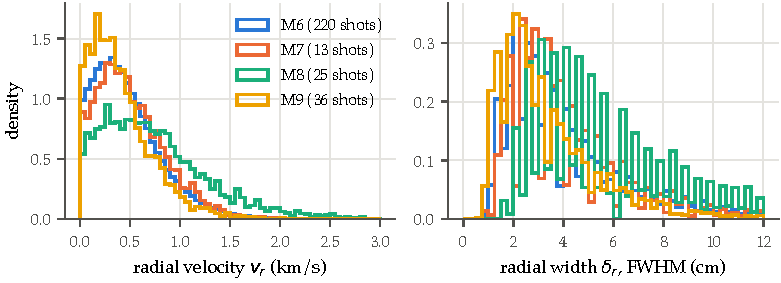
\includegraphics[width=\linewidth]{figs/fig_distributions.pdf}
\caption{Distributions of radial velocity (left) and radial FWHM (right) of the selected tracks in each campaign, pooled over the discharges in the statistics.}
\label{fig:distributions}
\end{figure}

\subsection{Independent velocity estimates}
Two estimates that do not use the tracking confirm the velocity scale, the first being the cross-correlation lag between the row-averaged fluctuation profiles of consecutive frames inside the near-edge window, which involves no detection step and gives a per-discharge median velocity of \xcorrVMed{}~m/s over the \nXcorr{} discharges in which more than half the frame pairs have a usable correlation peak. Its ratio to the tracking median is \xcorrRatioMed{} (\xcorrRatioLo--\xcorrRatioHi), and the two correlate across discharges with Spearman $\rho = \xcorrShotRho$, while a ratio below one is expected because the lag method weights every bright structure in the window, including the slow inboard part of the streaks and the stationary limb. The second, Lucas--Kanade flow at the detections, correlates with the track velocities within discharges, with a median per-discharge correlation of \lkAgreeMed{} and $\rho = \lkShotRho$ between discharge medians, but is smaller by a factor of \lkRatioMed. Because the streaks are elongated and inclined, the brightness-constancy constraint fixes only the component of motion normal to the streak, and displacements exceed one pixel per frame, both of which bias the flow magnitude down, so the flow serves only as a check on sign and ordering.
